	%!TEX root = ../../Main.tex
\graphicspath{{Chapters/Krav/}}
%-------------------------------------------------------------------------------

\chapter{Krav}
I dette afsnit beskrives kravene til hvilken funktionalitet systemet har. 


I samarbejde med vejleder er der opstillet en række krav.
\begin{itemize}
\item Systemets skal kunne filtrere en støj fra et lydsignal, som indeholder et tale signal overlappet af et støjsignal.
\item Brugeren skal manuelt kunne tænde og slukke for filtreringen.
\item Lydsignalet skal feedes til en højtaler som afspiller lyden fra mikrofonen. 
\end{itemize}

Kravene er bygget op gennem use cases, som beskriver systemets funktionelle krav, samt en liste over alle ikke-funktionelle krav for systemet. Først vises aktørbeskrivelserne
med tilhørende aktørkontekst diagram. Herefter vises use cases for systemet. Der er udfærdiget to use cases
der tilsammen beskriver funktionaliteten af systemet. I use case afsnittet vises der også et use case diagram
med alle use cases og hvordan aktørerne interagerer med dem. Til sidst gives et kort overblik over ikke funktionelle krav.

\section{Aktørbeskrivelse}

\begin{figure}[H]
	\centering
	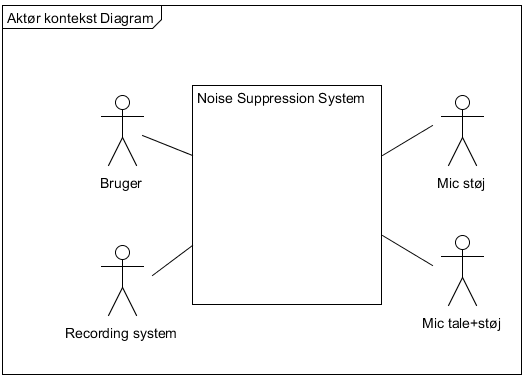
\includegraphics[width = 200 pt]{Img/Aktoer_Kontekst.png}
	\caption{Aktør Kontekst diagram}
	\label{fig:Aktoer Kontekst diagram}
\end{figure}

På figur \ref{fig:Aktoer Kontekst diagram} ses aktør kontekst diagrammet som beskriver sammenhængen mellem aktøren og det system den interagere med. Aktøren er som følger: \\*

\textbf{Bruger:} Den aktør der interagerer med systemet og vælger den ønskede funktionalitet \\


\section{Use case beskrivelse}

\begin{figure}[H]
	\centering
	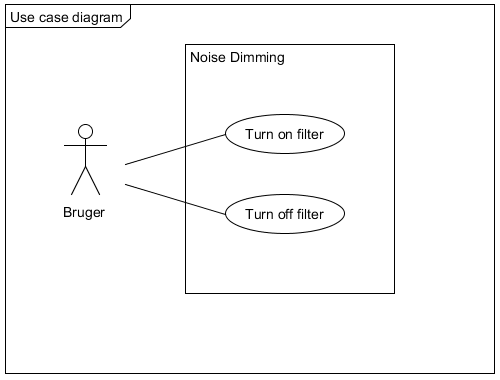
\includegraphics[width = 300 pt]{Img/Usecase_Diagram.png}
	\caption{Usecase diagram}
	\label{fig:Usecase diagram}
\end{figure}

På figur \ref{fig:Usecase diagram} ses usecase diagrammet som beskriver sammenhængen mellem aktørerne og de forskellige funktionaliteter der findes for systemet.

\subsubsection{UC 1 - Turn on filter}
Denne use case danner ramme for, at opfylde magasinet installeret på BFG. Brugeren interagerer med systemet, når han fylder magasinet. Brugeren får besked når magasinet er tomt, herefter åbnes og og genfyldes magasinet. Når brugeren har fyldt magasinet, godkender brugeren på GUI'en. Herefter lukker magasinet og genlader. 

\subsubsection{UC 2 - Turn off filter}
Denne use case danner ramme for manual styring af BFG. Brugeren interagere med systemet, når der trykkes på en retning i GUI'en. Brugeren har derudover mulighed for at affyre et projektil ved brug af "Skyd!"-knappen i GUI'en.  



\newpage
\section{Ikke-funktionelle krav}
Der er formuleret 12 ikke-funktionelle krav, som beskriver krav til selve systemets specifikation, ydeevne og kvaliteter. Disse kan alle måles eller visuelt observeres.
\begin{enumerate}
	\item Systemet skal have 2 mikrofoner og 1 højtaler
	
	\item Filteret skal gøre brug af LMS algoritmen
	
	\item Drejemekanismen skal kunne dreje horisontalt $\pm90^\circ$ om sin egen akse.
	
	\item Drejemekanismen skal kunne dreje minimum $5^\circ$ per sekund i horisontalt retning
	
	\item Affyringsmekanismen skal kunne skyde minimum 10 meter.
	
	\item Affyringsmekanismen skal kunne skyde minimum 2 gange i minuttet.
	
	\item Affyringsmekanismen skal have mulighed for præcis 6 projektiler i sit magasin af gangen.
	
	\item Affyringsmekanismen med stativ skal være minimum 1 meter og maximum 2 meter høj.
	
	\item Systemet skal gøre brug af pålidelig transmission mellem PC og selve affyringsmekanismen.
	
	\item Systemet skal have en brugergrænseflade på en PC med en mus/joystick/tastatur tilkoblet.
	
	
	\item Systemet skal kunne registrere og sigte automatisk efter objekter med én følgende farver: grøn, rød og blå.
	
	\item Systemets affyringsmekanisme skal køre på et batteri, som skal kunne holde til minimum 10 skud.
\end{enumerate}


\section{Acceptest}
Til hver use case er der lavet en tilhørende accepttest, der tjekker om use casen bliver gennemført korrekt. Udover de tre accepttests er der oprettet en accepttest af de ikke-funktionelle krav til systemet. Alle accepttests kan ses
i kravspecifikations dokumentation.